\chapter{Object Recognition}
\label{cha:objrecog}

\begin{chapterabstract}
In this chapter, we address the problem of object class recognition. To approach this challenge, we rely on the geometric information provided by 3D object representations such as point clouds. Furthermore, we focus on learning-based methods to distinguish objects from different classes while capturing the variability of shape of different objects which belong to the same class. More specifically, we leverage deep learning for such task. The chapter begins introducing and formulating the object recognition task in Section \ref{cha:objrecog:sec:introduction} followed by a review of the most relevant literature and datasets in Sections \ref{cha:objrecog:sec:relatedworks} and \ref{cha:objrecog:sec:datasets}. After that, we present our first proposal for 3D object recognition, namely PointNet, in Section \ref{cha:objrecog:sec:pointnet}. Later, PointNet is improved and thoroughly tested in adverse conditions with noise and occlusion throughout the study in Section \ref{cha:objrecog:sec:study}. Next, LonchaNet is introduced in Section \ref{cha:objrecog:sec:lonchanet} as the last iteration of our system that incorporates all the lessons learned by the previous work. Finally, Section \ref{cha:objrecog:sec:conclusion} draws conclusions and sets future lines of research.
\end{chapterabstract}

\section{Introduction}
\label{cha:objrecog:sec:introduction}

Object recognition is fundamental to computer vision and despite the progress achieved during the last years, it still remains a challenging area of research. Arguably, most of the interest in object recognition is due to its usefulness for robotics.

In that regard, recognizing objects is one of the problems that must be solved to achieve total visual scene understanding. Such deeper and better knowledge of the environment eases and enables the execution of a wide variety of more complex tasks. For instance, accurately recognizing objects in a room can be extremely useful for any robotic system that navigates within indoor environments. Due to the unstructured nature of those environments, autonomous robots need to do reasoning grounded in the dynamic real world. In other words, they need to understand the information captured by their sensors to perform tasks such as grasping, navigation, mapping, or even providing humans with information about their surroundings. Identifying the classes to which objects belong is one key step to enhance the aforementioned capabilities.

Despite the easy intuitive interpretation of the problem, its inherent difficulty can be misleading. We humans recognize numerous objects in difficult settings (e.g., different points of view, occlusion, or clutter) with little to no effort. However, approaching that problem is not that easy for a computer and taking into account all the possible settings and combinations of external factors renders this task a difficult one to solve efficiently and with high precision (which is often required in numerous application scenarios).

From a formal point of view, the object recognition task can be formulated as follows: given an image $\mathcal{I}^{H\times W}$ in which an object $\mathcal{O}$ appears, which can be either a gray-scale or RGB array of $W$ pixels in width and $H$ pixels in height, the goal is to predict the class of the object $\mathcal{L_O}$ from a set of $N$ predefined object classes $\mathcal{L} = \{\mathcal{L}_0, \mathcal{L}_1, ..., \mathcal{L}_{N-1}\}$.

Most of the classic literature of this topic tackled such problem by devising hand-crafted feature descriptors that are extracted on certain keypoints detected over the bidimensional image and later used either to compare them against pre-existing object descriptors in a database to match them to a certain class or either to feed them as input to a shallow machine learning architecture that learns to classify those descriptors to predict the class of the object that appears in the image. That paradigm shifted recently due to the success of deep learning architectures that are able to exploit their feature learning capabilities to avoid the need of hand engineering descriptors while achieving unprecedented accuracy levels. Furthermore, the adoption and spread of depth sensors has also added a literally new dimension to learn from to boost performance. The approaches introduced in this thesis are part of that cutting-edge trend that takes advantage of the additional geometric information facilitated by commodity range scanners to perform learning over them using deep architectures. A more detailed review of the field, from the very beginning to the current trends using 3D data and deep neural networks, is performed in Section \ref{cha:objrecog:sec:relatedworks}.

After that literature review, we start describing our first approach to perform object recognition using 3D data, namely PointNet, capable of learning object classes from point clouds discretized as occupancy grids with uniform voxel grids in the tridimensional space. Section \ref{cha:objrecog:sec:pointnet} describes this architecture, its data representation, and also benchmarks it on a standard 3D object classification dataset (ModelNet) to validate it.

Following that, Section \ref{cha:objrecog:sec:study} analyzes how noise and occlusion impact such 3D deep learning architecture and the importance of the data representation when dealing with such adverse conditions that commonly appear in the real world. In that study, we also propose minor changes to the architecture and the representation themselves that significantly boost accuracy with regard to the originally proposed PointNet.

At last, Section \ref{cha:objrecog:sec:lonchanet} takes all the lessons learned from the initial PointNet proposal and the extensive study to introduce a novel slice-based architecture to tackle the 3D object class recognition problem, LonchaNet, which achieved state of the art results in the aforementioned benchmark (ModelNet10).

\clearpage

\section{Related Works}
\label{cha:objrecog:sec:relatedworks}

\subsection{2D Object Recognition}
\label{cha:objrecog:sec:relatedworks:subsec:2d}

\subsection{RGB-D Object Recognition}
\label{cha:objrecog:sec:relatedworks:subsec:rgbd}

\subsection{3D Object Recognition}
\label{cha:objrecog:sec:relatedworks:subsec:3d}

\section{Datasets}
\label{cha:objrecog:sec:datasets}

% TODO: Introductory paragraph

In order to evaluate the performance of our proposal in terms of accuracy we made extensive use of a well-known dataset such as the Princeton ModelNet project [REF]. Its goal, as their authors state, is to provide researchers with a comprehensive clean collection of 3D \ac{CAD} models for objects, which were obtained via online search engines. Employees from the Amazon Mechanical Turk service were hired to classify over $150,000$ models into $662$ categories.

At the moment, there are two versions of this dataset publicly available for download 2 : ModelNet-10 and ModelNet-40. Those are subsets of the original dataset, only providing the $10$ and $40$ most popular object categories respectively. They are specially clean since the models that did not belong to the specified categories were manually deleted.

On the one hand, ModelNet-10 is composed of a collection of over $5,000$ \ac{CAD} models classified into $10$ categories and divided into training and test sets. In addition, the orientation of all the \ac{CAD} models was manually aligned. On the other hand ModelNet-40 features over $9,800$ models classified into $40$ categories and it also includes training and test splits; however, their orientations are not aligned as they are in ModelNet-10.

\section{PointNet}
\label{cha:objrecog:sec:pointnet}

The proposed system takes a point cloud of an object as an input and predicts its class label. In this regard, the proposal is twofold: a volumetric grid based on point density to estimate spatial occupancy inside each voxel, and a pure \ac{3D}-\ac{CNN} which is trained to predict object classes. The occupancy grid -- inspired by VoxNet \cite{Maturana2015} occupancy models based on probabilistic estimates -- provides a compact representation of the object's 3D information from the point cloud. That grid is fed to the \ac{CNN} architecture, which in turn computes a label for that sample, i.e., predicts the class of the object.

\subsection{Data Representation}
\label{cha:objrecog:sec:pointnet:subsec:data}

As we mentioned before, our proposed architecture takes a point cloud of an object as input to recognize it. However, point clouds are unstructured representations that cannot be easily handled by common \ac{CNN} architectures due to the lack of a matrix-like organization. The most straightforward way to apply formal convolutions to that unstructured space is to impose a certain organization into it.

Occupancy grids are data structures which allow us to obtain a compact representation of the volumetric space. They stand between meshes or clouds, which offer rich but large amounts of information, and voxelized representations with packed but poor information. At that midpoint, occupancy grids provide considerable shape cues to perform learning, while enabling an efficient processing of that information thanks to their array-like implementation.

% TODO: Talk about other approaches that make use of occupancy grids

With PointNet, we propose an occupancy grid inspired by the aforementioned successes but aiming to maintain a reasonable accuracy while allowing a real-time implementation. In our volumetric representation, each point of a cloud is mapped to a voxel of a fixed-size occupancy grid. Before performing that mapping, the object cloud is scaled to fit the grid. Each voxel will hold a value representing the number of points mapped to itself. At last, the values held by each cell are normalized. Figure \ref{fig:objrecog:meshcloudgrid} shows the derivation of the proposed occupancy grid representation from other typical tridimensional representations of a sample object.

\begin{figure}
  \centering
  \begin{subfigure}{0.3\linewidth}
    \centering
    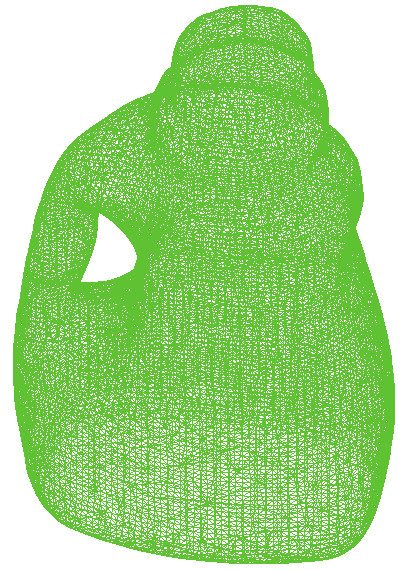
\includegraphics[width=\linewidth]{Figures/ObjRecog/mesh.png}
    \caption{Mesh}
    \label{fig:objrecog:meshcloudgrid:mesh}
  \end{subfigure}
  \begin{subfigure}{0.3\linewidth}
    \centering
    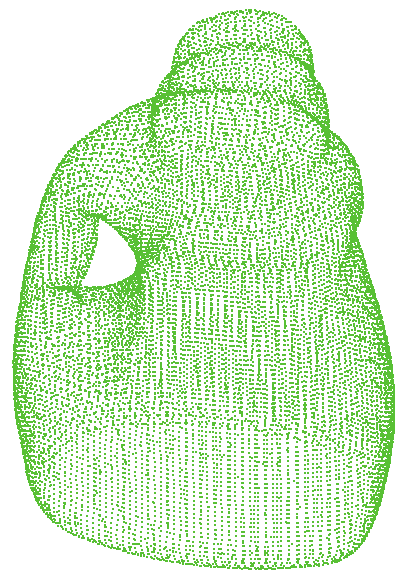
\includegraphics[width=\linewidth]{Figures/ObjRecog/cloud.png}
    \caption{Cloud}
    \label{fig:objrecog:meshcloudgrid:cloud}
  \end{subfigure}
  \begin{subfigure}{0.3\linewidth}
    \centering
    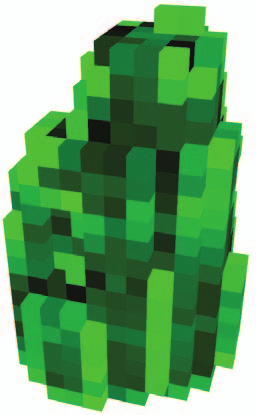
\includegraphics[width=0.9\linewidth]{Figures/ObjRecog/grid.png}
    \caption{Grid}
    \label{fig:objrecog:meshcloudgrid:grid}
  \end{subfigure}
  \caption{Various 3D representations for an object. A mesh (\subref{fig:objrecog:meshcloudgrid:mesh}) is transformed into a point cloud (\subref{fig:objrecog:meshcloudgrid:cloud}), and that cloud is processed to obtain a voxelized occupancy grid (\subref{fig:objrecog:meshcloudgrid:grid}). The occupancy grid shown in this figure is a cube of $30\times 30 \times 30$ voxels. Each voxel of that cube holds the point density inside its volume. In this case, dark voxels indicate high density whilst bright ones are low density volumes. Empty voxels were removed for better visualization.}
  \label{fig:objrecog:meshcloudgrid}
\end{figure}

\subsection{Network Architecture}
\label{cha:objrecog:sec:pointnet:subsec:network}

\subsection{Experiments}
\label{cha:objrecog:sec:pointnet:subsec:experiments}

This architecture was implemented using the Point Cloud Library (PCL) [23] – which contains state-of-the-art algorithms for 3D point cloud processing – and Caffe [19], a deep learning framework developed and maintained by the Berkeley Vision and Learning Center (BVLC) and an active community of contributors on GitHub 1. This BSD-licensed C++ library allows us to design, train, and deploy CNN architectures efficiently, mainly thanks to its drop-in integration of NVIDIA cuDNN [24] to take advantage of GPU acceleration.

\subsubsection{Methodology}

The CAD models are provided in Object File Format (OFF). Firstly, we converted all OFF models into Polygon File Format (PLY) to ease the usage of the dataset with the PCL. As we already mentioned, the input for PointNet are point clouds, but the dataset provides CAD models specifying vertices and faces. In this regard, we converted the PLY models into Point Cloud Data (PCD) clouds by raytracing them. A 3D sphere is tessellated and a virtual camera is placed in each vertex of that truncated icosahedron – pointing to the origin of the model – then multiple snapshots are rendered using raytracing and the z-buffer data, which contains the depth information, is used to generate point clouds from each point of view. After all points of view have been processed, the point clouds are merged. A voxel grid filter is applied to downsample the clouds after the raytracing operations. Figure 3 illustrates the aforementioned processes. After that, the resulting point clouds are used to train, randomizing the order of the models, and test the system taking into account the corresponding splits.

All the timings and results were obtained by performing the experiments in the following test setup: Intel Core i5-3570 with 8 GB of 1600 MHz DD3 RAM on an ASUS P8H77-M PRO motherboard (Intel H77 chipset). Additionally, the system includes an NVIDIA Tesla K20 GPU, and a Seagate Barracuda 7200.14 secondary storage. Caffe RC2 was run over ElementaryOS Freya 0.3.1, an Ubuntu-based Linux distribution. It was compiled using CMake 2.8.7, g++ 4.8.2, CUDA 7.0, and cuDNN v3.

% TODO: Source code

\subsection{Discussion}
\label{cha:objrecog:sec:pointnet:subsec:discussion}

\section{Noise and Occlusion}
\label{cha:objrecog:sec:study}

\section{LonchaNet}
\label{cha:objrecog:sec:lonchanet}

\section{Conclusion}
\label{cha:objrecog:sec:conclusion}
